\section{\label{sec:group_structure}Group structure of space groups}

\subsection{\label{sec:def_space_group}Definition of space group}

Let $f$ be a crystal pattern.
A space group of $f$ is defined as the stabilizer on $\mathcal{E}_{n}$.

\begin{screen}
  \begin{defn}[space group]
    The stabilizer of crystal pattern $f$ on $\mathcal{E}_{n}$
    \begin{align}
      \mathcal{G} \coloneqq \mathrm{Stab}_{\mathcal{E}_{n}} (f) = \set{ g \in \mathcal{E}_{n} }{ g f = f }
    \end{align}
    is called \term{space group} if $\mathcal{T}(\mathcal{G}) \coloneqq \mathcal{T}_{n} \cap \mathcal{G}$ is isomorphic to a $n$-dimensional lattice.
    For the space group $\mathcal{G}$, $\mathcal{T}(\mathcal{G})$ is called \term{translation subgroup} of $\mathcal{G}$.
  \end{defn}
\end{screen}

The above definition is for space groups in a broad sense.
In a narrow sense, the space group of a stabilizer of a three-dimensional crystal pattern with a three-dimensional translational subgroup.
The other symmetry groups for crystal patterns are summarized in Table~\ref{tab:symmetry_groups}.

\begin{table}[htb]
  \centering
  \caption{Symmetry groups of $n$-dimensional crystal patterns with $r$-dimensional translations.}
  \label{tab:symmetry_groups}
  \begin{tabular}[h]{cccc}
    \hline\hline
    $n$ & $r$ & Symmetry group & Table \\
    \hline
    2 & 1 & Frieze group & Section 2.1 of ITE \cite{ITE2010} \\
    2 & 2 & Plane group  & Section 2.2 of ITA \cite{ITA2016} \\
    3 & 1 & Rod group    & Section 3.1 of ITE \cite{ITE2010} \\
    3 & 2 & Layer group  & Section 4.1 of ITE \cite{ITE2010} \\
    3 & 3 & Space group  & Section 2.3 of ITA \cite{ITA2016} \\
    \hline\hline
  \end{tabular}
\end{table}

\subsection{Point group}

Let $\mathcal{G}$ be a space group.
The translation subgroup $\mathcal{T}(\mathcal{G})$ is normal subgroup of $\mathcal{G}$:
For any $ (\mathbf{W}, \mathbf{w}) \in \mathcal{G}$ and $(\mathbf{I}_{n}, \mathbf{t}) \in \mathcal{T}(\mathcal{G})$, one has
\begin{align}
  (\bm{W}, \bm{w}) (\bm{I}_{n}, \bm{t}) (\bm{W}, \bm{w})^{-1} = (\bm{I}_{n}, \bm{Wt}) \in \mathcal{T}(\mathcal{G}).
\end{align}

\begin{screen}
  \begin{defn}[point group]
    The set of the linear parts of a space group $\mathcal{G}$ is called \term{point group} of $\mathcal{G}$
    \begin{align}
      \mathcal{P}(\mathcal{G}) \coloneqq \set{ \mathbf{W} }{ (\bm{W}, \bm{w}) \in \mathcal{G} }.
    \end{align}
    The point group $\mathcal{P}(\mathcal{G})$ is isomorphic to the factor group $\mathcal{G} / \mathcal{T}(\mathcal{G})$.
  \end{defn}
\end{screen}

The homomorphism $\mathcal{G} \ni (\bm{W}, \bm{w}) \mapsto \bm{W} \in \mathcal{P}(\mathcal{G})$ gives the isomorphism between $\mathcal{G} / \mathcal{T}(\mathcal{G})$ and $\mathcal{P}(\mathcal{G})$.

We fix some basis vectors $(\bm{a}_{1}, \dots, \bm{a}_{n})$ of affine space, and act all mappings in point group $\mathcal{P}$ on the basis vectors.
Since affine mappings in the point group $\mathcal{P}$ are isometry, it does not change the norm of vectors.
Therefore, there are only finitely many acted vectors because the maximum norm of acted vectors is bound by $\max_{i=1,\dots,n} \mathbf{a}_{i}$.

\begin{screen}
  \begin{them}
    The point group $\mathcal{P}$ of a space group $\mathcal{G}$ is finite.
  \end{them}
\end{screen}

When we choose the lattice basis of $\mathcal{T}(\mathcal{G})$ as the basis vectors of the affine spaces, the translation subgroup $\mathcal{T}(\mathcal{G})$ is represented as $\set{ (\bm{I}_{n}, \bm{t}) }{ \bm{t} \in \mathbb{Z}^{n} }$.
And the action of point group $\mathcal{P}$ is described as integer matrices.

\begin{figure}[tb]
  \centering
  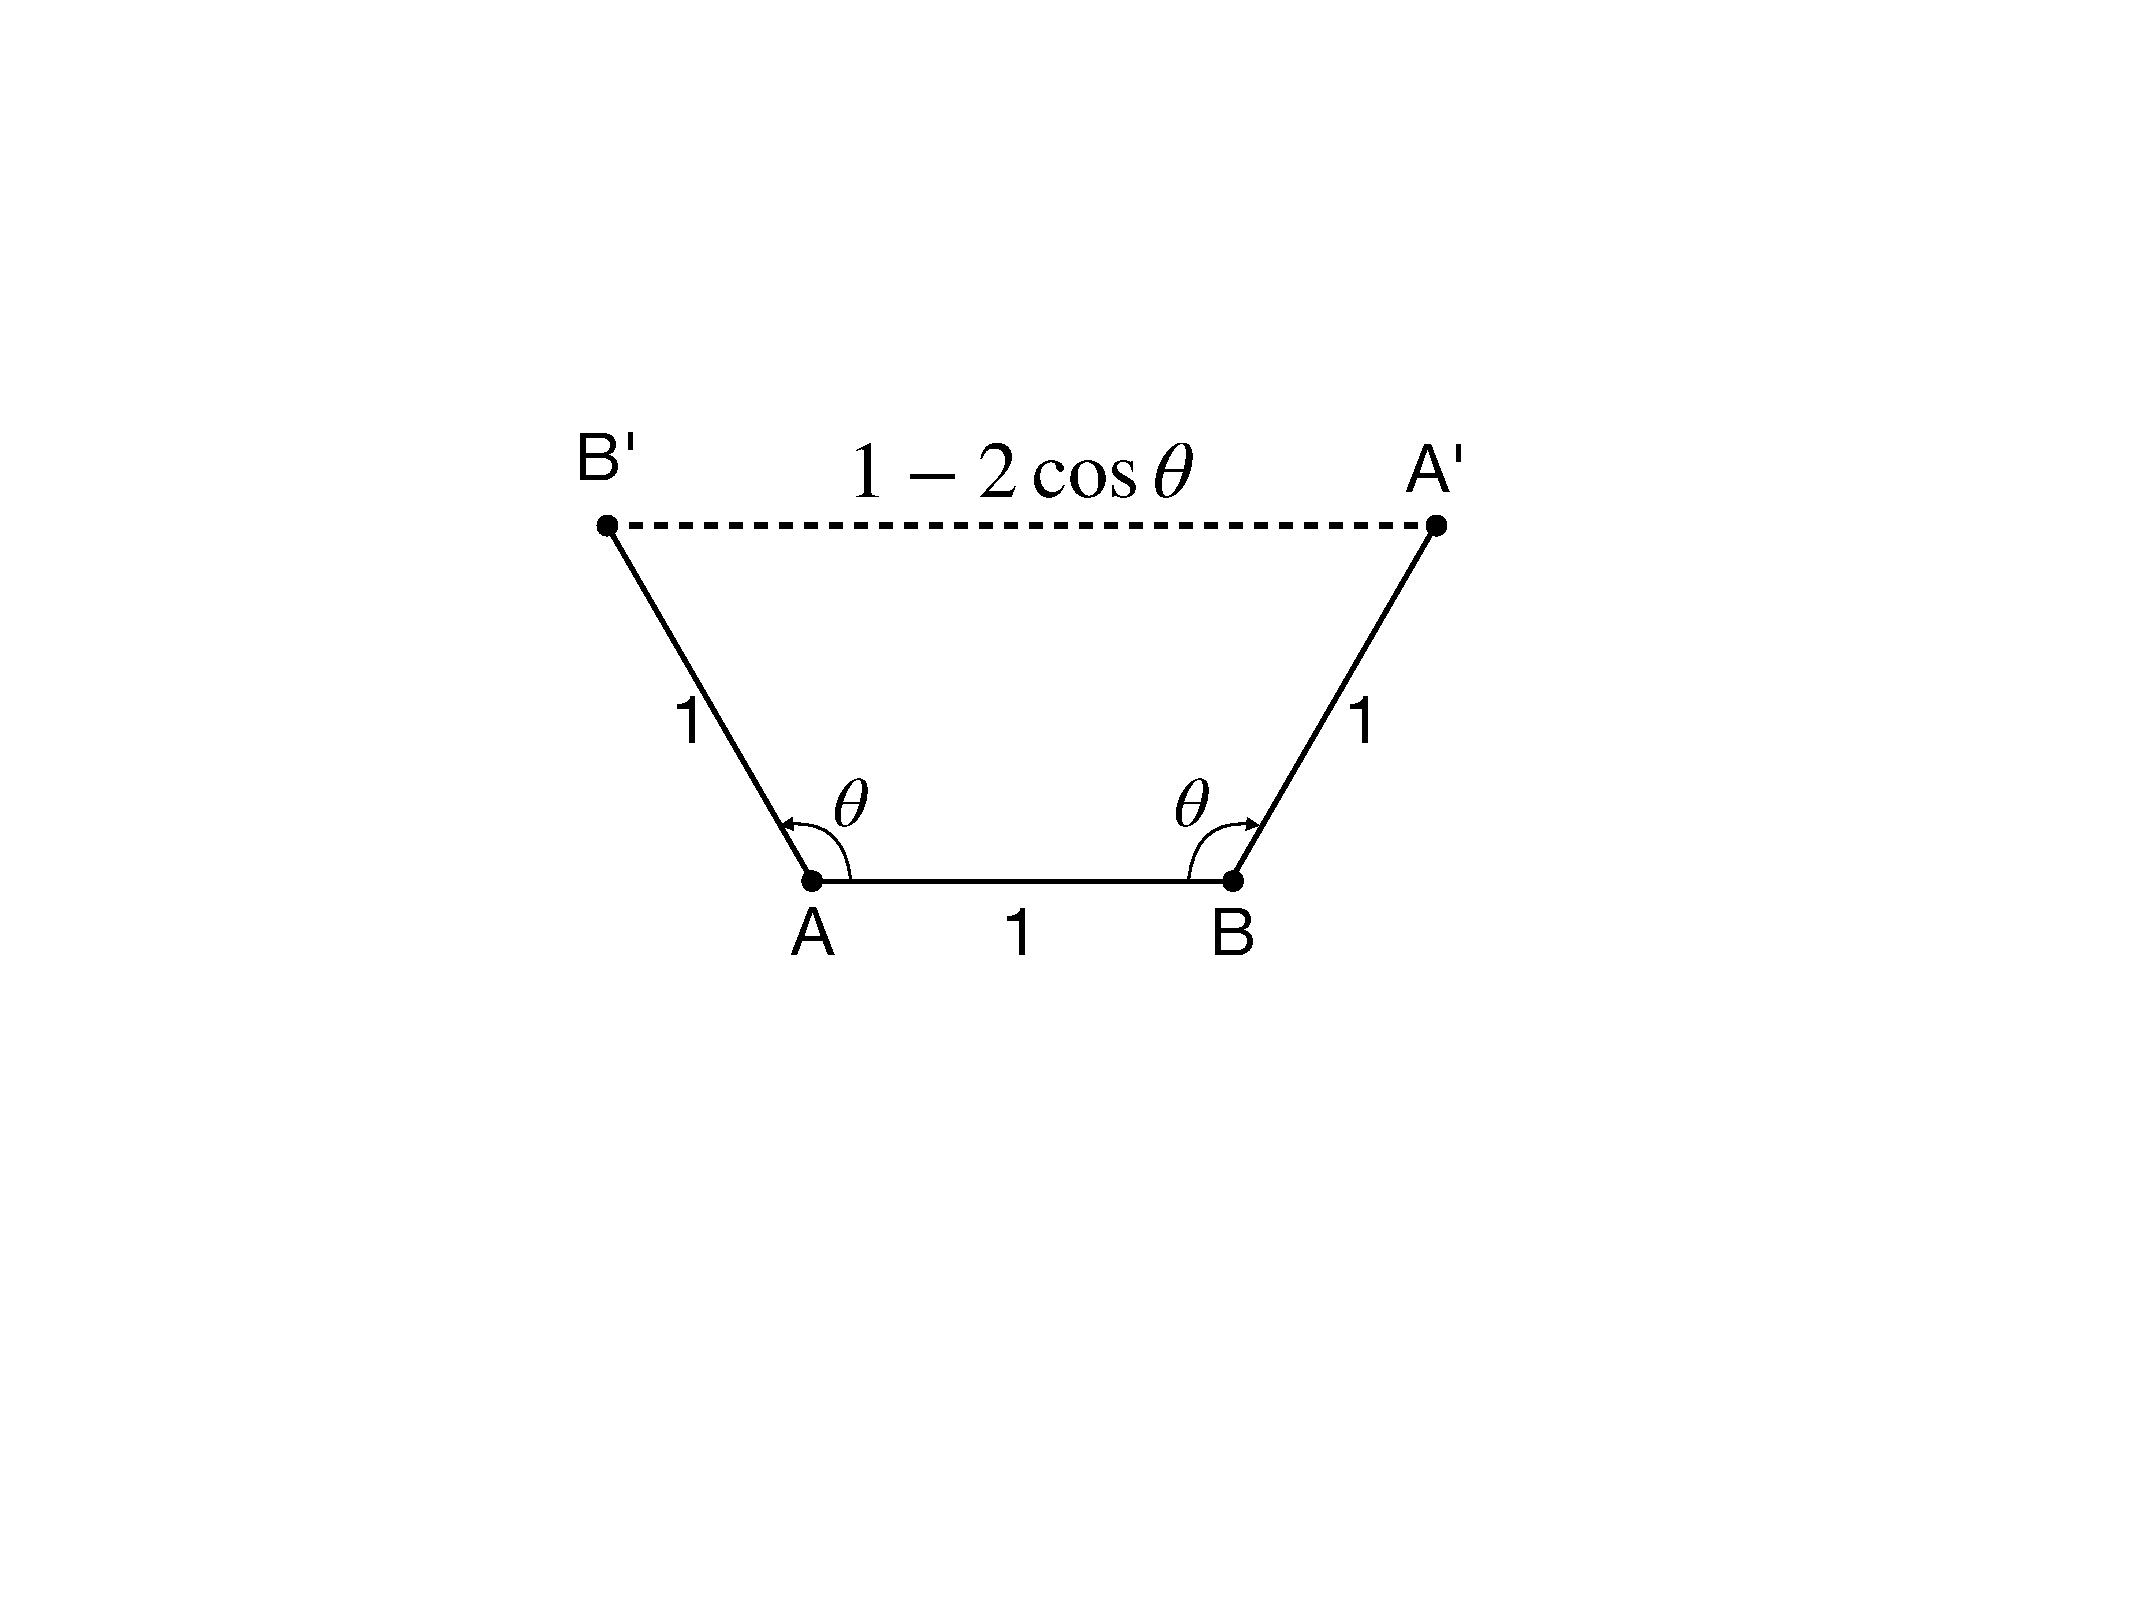
\includegraphics[width=0.5\textwidth]{figure/fig_crystallographic_rotation_3d.pdf}
  \caption{Rotations acting on a lattice are 1, 2, 3, 4, or 6 fold rotations.}
  \label{fig:crystallographic_rotation_3d}
\end{figure}

In particular, proper rotations of a point group of a three-dimensional space group should be 1, 2, 3, 4, or 6 fold rotations.
The proof is sketched in Fig.~\ref{fig:crystallographic_rotation_3d}.
We pick a lattice point $A$ and its nearest lattice point $B$\footnote{
  Because a lattice is discrete, $A$ and $B$ are distinct points, $A \neq B$.
}.
For simplicity, we scale the length between $A$ and $B$ to be one.
When we consider a $n$-fold rotation with angle $\theta = \frac{2\pi}{n}$, the rotation with origin $A$ maps $B$ to $B'$, and the rotation with origin $B$ maps $A$ to $A'$.
Then, the length between $A'$ and $B'$, $A'B' = 1 - 2 \cos \theta$ should be an integer because lengths between lattice points should be multiple of $AB=1$.
Thus, $\cos \theta$ should be one of $1, -1, \frac{1}{2}, 0, -\frac{1}{2}$ and these rotations correspond to 1, 2, 3, 4, and 6 fold rotations.
For an improper rotation $\bm{W}$ with $\det \bm{W} < 0$, the corresponding proper rotation $-\bm{W}$ should also be 1, 2, 3, 4, or 6 fold rotations.

\subsection{\label{sec:vector_system}Symmorphic and non-symmorphic space groups}

The translation subgroup of space group $\mathcal{G}$ can be chosen to be $\mathcal{T} = \mathbb{Z}^{n}$ by choosing primitive basis vectors.
Also, the point group of $\mathcal{G}$ is a finite subgroup $\mathcal{P}$ of $\mathrm{GL}(n, \mathbb{Z})$.
In general, a space group is not specified only with the translation subgroup $\mathcal{T}$ and point group $\mathcal{P}$.
We need to determine a translation part $\bm{\tau}(\bm{W})$ of each linear part $\bm{W} \in \mathcal{P}$.
We can construct $\mathcal{G}$ from $\mathcal{T}$, $\mathcal{{P}}$, and $\bm{\tau}$ as
\begin{align}
  \mathcal{G} = \set{
    \begin{pmatrix}
      \bm{W} & \bm{\tau}(\bm{W}) + \bm{t} \\
      \bm{0}^{\top} & 1 \\
    \end{pmatrix}
  } {
    \bm{W} \in \mathcal{P}, \bm{t} \in \mathbb{Z}^{n}
  }.
\end{align}

Because the addition of lattice translation into $\bm{\tau}$ gives the same space group, it is sufficient to confine the range of $\bm{\tau}$ as $\bm{\tau}: \mathcal{P} \to [0, 1)^{n}$.
Furthermore, the map $\bm{\tau}$ should satisfy a \term{cocycle condition}
\begin{align}
  \label{eq:cocycle_condition}
  \bm{\tau}(\bm{W}\bm{W}') \equiv \bm{\tau}(\bm{W}) + \bm{W} \bm{\tau}(\bm{W}') \quad ( \mathrm{mod} \, \mathbb{Z}^{n})
\end{align}
for all $\bm{W}, \bm{W}' \in \mathcal{P}$ so that a vector system consistent with the product of two symmetry operations:
\begin{align*}
  \begin{pmatrix}
    \bm{W} & \bm{\tau}(\bm{W}) \\
    \bm{0}^{\top} & 1
  \end{pmatrix}
  \begin{pmatrix}
    \bm{W}' & \bm{\tau}(\bm{W}') \\
    \bm{0}^{\top} & 1
  \end{pmatrix}
  =
  \begin{pmatrix}
    \bm{W}\bm{W}' & \bm{\tau}(\bm{W}) + \bm{W} \bm{\tau}(\bm{W}') \\
    \bm{0}^{\top} & 1
  \end{pmatrix}.
\end{align*}
In particular, the cocycle condition for $\bm{I}_{n}$ and $\bm{I}_{n}$ gives $\bm{\tau}(\bm{I}_{n}) \equiv \bm{0} \, (\mathrm{mod}\, \mathbb{Z}^{n})$.

\begin{screen}
  \begin{defn}[vector system \cite{Eick2005}]
    Let $\mathcal{P}$ be a point group of a space group $\mathcal{G}$.
    The map $\bm{\tau}: \mathcal{P} \to \mathbb{R}^{n}$ is called a \term{vector system} if the map satisfies \term{cocycle condition} in Eq.~\eqref{eq:cocycle_condition}.
  \end{defn}
\end{screen}
In summary, a space group is fully constructed from its translation subgroup, point group, and vector system.

Note that the choice of the origin of the affine space transforms the translation part $\bm{\tau}$.
When we change the origin from $\bm{O}$ to $\bm{O} + \bm{Ap}$, a symmetry operation $(\bm{W}, \bm{\tau}(\bm{W}))$ are transformed to
\begin{align*}
  \begin{pmatrix}
    \bm{I}_{n} & \bm{p} \\
    \bm{0}^{\top} & 1 \\
  \end{pmatrix}^{-1}
  \begin{pmatrix}
    \bm{W} & \bm{\tau}(\bm{W}) \\
    \bm{0}^{\top} & 1 \\
  \end{pmatrix}
  \begin{pmatrix}
    \bm{I}_{n} & \bm{p} \\
    \bm{0}^{\top} & 1 \\
  \end{pmatrix}
  =
  \begin{pmatrix}
    \bm{W} & \bm{\tau}(\bm{W}) + (\bm{W} - \bm{I}_{n})\bm{p} \\
    \bm{0}^{\top} & 1 \\
  \end{pmatrix}
\end{align*}
from Eq.~\eqref{eq:operation_transformation}.
Thus, for any $\bm{p} \in \mathbb{R}^{n}$, a vector system
\begin{align}
  \bm{\tau}_{\bm{p}}(\bm{W})
    \coloneqq \bm{\tau}(\bm{W}) + (\bm{W} - \bm{I}_{n}) \bm{p}
    \quad (\bm{W} \in \mathcal{P})
\end{align}
and $\bm{\tau}$ give the same space group.

\begin{screen}
  \begin{defn}[symmorphic and non-symmorphic]
    Let $\bm{\tau}$ be a vector system of a space group $\mathcal{G}$.
    If there exists an origin shift $\bm{p} \in \mathbb{R}^{n}$ such that $\bm{\tau}_{\bm{p}} \equiv \bm{0}$, $\mathcal{G}$ is called a \term{symmorphic} space group.
    Otherwise, $\mathcal{G}$ is called a \term{non-symmorphic} space group.
  \end{defn}
\end{screen}

\subsection{Working examples from plane groups}

Let us derive plane groups $p2mm$, $p2mg$ and $p2gg$ from a translation group $\mathbb{Z}^{2}$ and a point group
\begin{align*}
  \mathcal{P}_{\mathrm{2mm}} = \left\{
    \bm{W}_{0} = \begin{pmatrix}
      1 & 0 \\
      0 & 1 \\
    \end{pmatrix},
    \bm{W}_{1} = \begin{pmatrix}
      -1 & 0 \\
      0 & -1 \\
    \end{pmatrix},
    \bm{W}_{2} = \begin{pmatrix}
      -1 & 0 \\
      0 & 1 \\
    \end{pmatrix},
    \bm{W}_{3} = \begin{pmatrix}
      1 & 0 \\
      0 & -1 \\
    \end{pmatrix}
  \right\}.
\end{align*}
This example is adapted from Section 4.2 of Ref.~\cite{Souvignier08}.

Let $\bm{\tau}_{i} = \bm{\tau}(\bm{W}_{i})$ for $i = 1, \dots, 4$.
It is sufficient to consider $\bm{\tau}_{2} = \begin{pmatrix} a_{2} \\ b_{2} \end{pmatrix}$ and $\bm{\tau}_{3} = \begin{pmatrix} a_{3} \\ b_{3} \end{pmatrix}$ because the remains are obtained from the cocycle condition,
\begin{align*}
  \bm{\tau}_{1}
    &= \bm{\tau}(\bm{W}_{2}\bm{W}_{3})
    = \bm{\tau}_{2} + \bm{W}_{2} \bm{\tau}_{3}
    = \begin{pmatrix} a_{2} - a_{3} \\ b_{2} + b_{3} \end{pmatrix}.
\end{align*}
The relation $\bm{W}_{2}^{2} = \bm{W}_{0}$ gives
\begin{align*}
  \bm{\tau}_{0}
    &= \bm{\tau}(\bm{W}_{2}^{2})
    = \bm{\tau}_{2} + \bm{W}_{2} \bm{\tau}_{2}
    = \begin{pmatrix} 0 \\ 2 b_{2} \end{pmatrix} \\
  \therefore 2b_{2} &\equiv 0 \, (\mathrm{mod}\, \mathbb{Z}).
\end{align*}
The relation $\bm{W}_{3}^{2} = \bm{W}_{0}$ gives
\begin{align*}
  \bm{\tau}_{0}
    &= \bm{\tau}_{3} + \bm{W}_{3} \bm{\tau}_{3}
    = \begin{pmatrix} 2 a_{3} \\ 0 \end{pmatrix} \\
  \therefore 2 a_{3} &\equiv 0 \, (\mathrm{mod}\, \mathbb{Z}).
\end{align*}
The relation $(\bm{W}_{2}\bm{W}_{3})^{2} = \bm{W}_{1}^{2} = \bm{W}_{0}$ gives no restriction,
\begin{align*}
  \bm{\tau}_{0}
    &= \bm{\tau}_{1} + \bm{W}_{1} \bm{\tau}_{1}
    = \begin{pmatrix} 0 \\ 0 \end{pmatrix}.
\end{align*}

The trivial vector system $\bm{\tau}^{0}_{\bm{p}, i} = (\bm{W}_{i} - \bm{I}) \bm{p} \quad (i=1,\dots,4)$ for origin shift $\bm{p} = \begin{pmatrix} p \\ q \end{pmatrix}$ is computed as
\begin{align*}
  \bm{\tau}^{0}_{\bm{p}, 0} = \begin{pmatrix} 0 \\ 0 \end{pmatrix},
  \bm{\tau}^{0}_{\bm{p}, 1} = \begin{pmatrix} -2 p \\ -2 q \end{pmatrix},
  \bm{\tau}^{0}_{\bm{p}, 2} = \begin{pmatrix} -2 p \\ 0 \end{pmatrix},
  \bm{\tau}^{0}_{\bm{p}, 3} = \begin{pmatrix} 0 \\ -2 q \end{pmatrix}.
\end{align*}.
Thus, we can choose $p=-\frac{a_{2}}{2}, q=-\frac{b_{3}}{2}$ so that $a_{2} = b_{3} = 0$.
We derived the following vector systems
\begin{itemize}
  \item $\bm{\tau}_{2} = \bm{\tau}_{3} = \begin{pmatrix} 0 \\ 0 \end{pmatrix}$: $p2mm$
  \item $\bm{\tau}_{2} = \begin{pmatrix} 0 \\ 0 \end{pmatrix}, \bm{\tau}_{3} = \begin{pmatrix} \frac{1}{2} \\ 0 \end{pmatrix}$: $p2mg$ (reflection along $a$ axis and glide along $b$ axis)
  \item $\bm{\tau}_{2} = \begin{pmatrix} 0 \\ \frac{1}{2} \end{pmatrix}, \bm{\tau}_{3} = \begin{pmatrix} 0 \\ 0 \end{pmatrix}$: $p2mg$ (reflection along $b$ axis and glide along $a$ axis)
  \item $\bm{\tau}_{2} = \begin{pmatrix} 0 \\ \frac{1}{2} \end{pmatrix}, \bm{\tau}_{3} = \begin{pmatrix} \frac{1}{2} \\ 0 \end{pmatrix}$: $p2gg$.
\end{itemize}
